\section{Внешняя среда предприятия. Макроэкономика.\\Основы экономики.}

\subsection{Определение экономики}

\textbf{Экономика} -- это

\begin{enumerate}
    \item способ организации деятельности людей, напревленный на создание благ для удовлетворения их потребностей;
    \item наука, изучающая как удовлетворить максимальные растущие потребности людей при сокращающихся ресурсах.
\end{enumerate}

\subsection{Экономические отношения}

\begin{enumerate}
    \item \textbf{Социально-экономические} отношения обусловлены строением (устройством) общества, тем как он функционирует и взаимоотношениями между людьми
    \item \textbf{Организационно-экономические} отношения обусловлены общественным разделением труда

        \begin{enumerate}
            \item \textbf{Первичный сектор} -- отрасли, связанные с добычей полезных ископаемых (лесная, нефтегазовая, железодобывающая)
            \item \textbf{Вторичный сектор} -- отрасли переработки и производства
            \item \textbf{Третичный сектор} -- услуги (торговля), образование
            \item \textbf{Четверичный сектор} -- ифнормационные технологии
        \end{enumerate}

    \item \textbf{Управленчиские} отношения могут воникать по вертикали и горизонтали.
\end{enumerate}

\subsubsection{Субъекты экономических отношений}

\begin{enumerate}
    \item \textbf{Домохозяйтсво} -- единица общества, самостоятельно принимающая экономические решения.
    \item \textbf{Предприятие} (фирма) -- обладает самостоятельностью в принятии экономических решений, но при этом предприятие стремится производить продокцию (услуги) с учетом имеющихся ресурвом и фактором и продаже по наиболее высокой цене.
    \item \textbf{Государство} -- институт, совокупность государственных структур, которые имеют возможность и рисурсы при необхоимости оказывать воздейтвие на другие субъекты экономических отношений.
    \item \textbf{Некомерческие организации, партнерства, ассоциации и т.д.} -- могут отражать совокупность взглядов группы хозяйств, группы домохозяйств и предприятий, группы предприятий
\end{enumerate}

\subsection{Факторы производства}

\begin{enumerate}
    \item \textbf{Труд}
    \item \textbf{Земля}
    \item \textbf{Капитал}

        \begin{itemize}
            \item Основной -- то, чем предприятие владеет;
            \item Оборотный -- то, чт оиспользуется в течение одного производственного цикла
        \end{itemize}

    \item \textbf{Предпринимательские способности} -- умение организовать, рисковать, видеть перспективы и слабые места
\end{enumerate}

\begin{table}[H]
    \centering
    \begin{tabular}{|c|c|c|c|c|}
        \hline
            & Труд & Земля & Капитал & Предпринимательские способности \\
        \hline
        Доход & Зарплата & Рента & Процент & \\
        \hline
    \end{tabular}
\end{table}

\subsection{Модели экономических систем}

\subsubsection{Кривая предельных производственных возможностей}

Вопросы, которые решает экономика:

\begin{enumerate}
    \item Что производить
    \item Как производить
    \item Для кого производить
\end{enumerate}

\subsubsection{Модели экономики}

\begin{enumerate}
    \item Традиционная экономика
    \item Централизованно-управляемая (все решается государством)
    \item Рыночная экономика (конкурентный рынок)
    \item Смешанная модель (рынок + государство)
\end{enumerate}

\subsubsection{Рыночная экономика и ее отличительные признаки}

\subsubsection{Функции рынка}

\begin{enumerate}
    \item Ценообразования
    \item Информационная
    \item Стимулирующая
    \item Санирующая
    \item Регулирующая
\end{enumerate}

\subsubsection{Кругооборот благ (ресурсов) в рыночной экономике}

\begin{figure}[H]
    \centering
    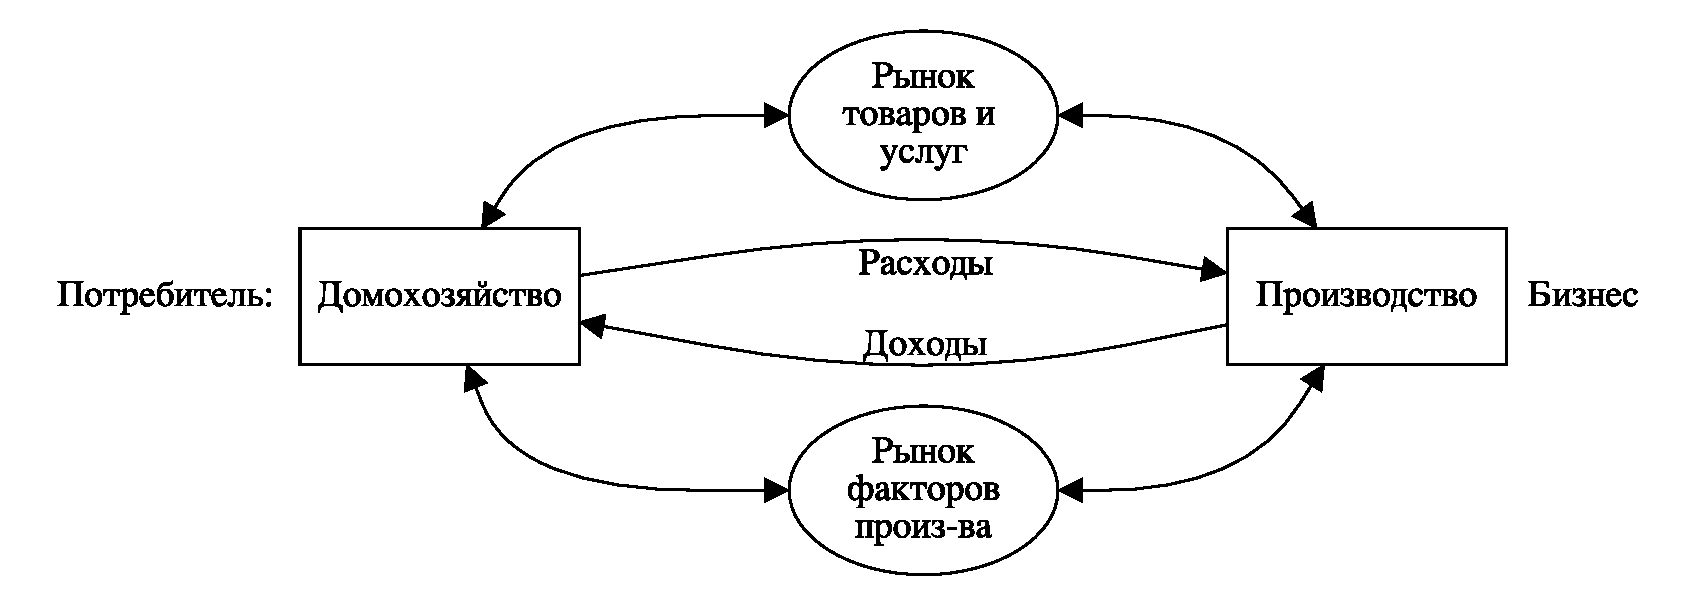
\includegraphics[width=0.8\textwidth]{img/content/module_1/circle.pdf}
    \label{fig:}
\end{figure}
